\documentclass{standalone}

\usepackage{pgfplots}

\pgfplotsset{compat=1.9}

\begin{document}
\pgfplotsset{domain=-5:5}

\begin{tikzpicture}
	\begin{axis}
	\addplot[
		variable=u,
	]
	{u^2};
	\end{axis}
\end{tikzpicture}
\begin{tikzpicture}
	\begin{axis}
	\addplot[
		variable=u,
	]
	(u,u^2);
	\end{axis}
\end{tikzpicture}

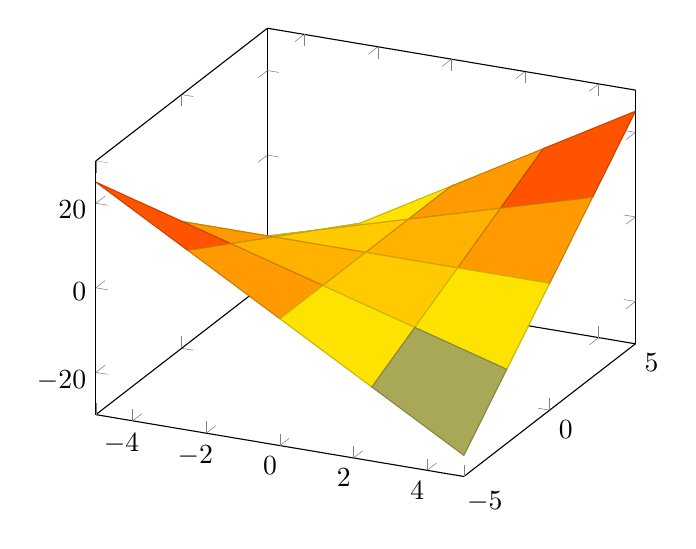
\begin{tikzpicture}
	\begin{axis}
	\addplot3[
		surf,
		samples=5,
		variable=u,
		variable y=v,
	]
	{u*v};
	\end{axis}
\end{tikzpicture}
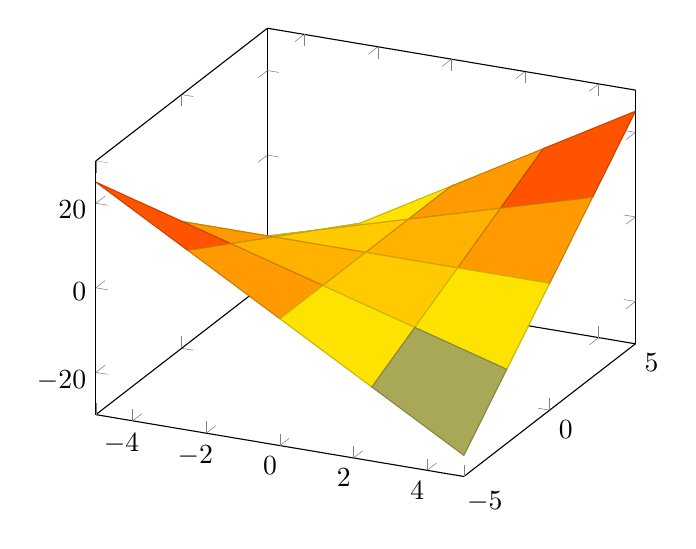
\begin{tikzpicture}
	\begin{axis}
	\addplot3[
		surf,
		samples=5,
		variable=u,
		variable y=v,
	]
	(u,v,u*v);
	\end{axis}
\end{tikzpicture}

\end{document}

